% \documentclass[handout]{beamer} %"handout" serveix per a treure els \pause
\documentclass{beamer} %"handout" serveix per a treure els \pause
\usepackage{preamble}
\usepackage{../bibliography}

\usetheme{Copenhagen}
\usecolortheme{seahorse}

%%%%%%%%%%%%%%%%%%%%%%%%%%%%%%%%%%%%%%%%%%%%%%%%%%%%%%%%%%%%%%%%%%%%%%%%%%%%%%
% \embedvideo{<poster or text>}{<video file (MP4+H264)>}
% \embedvideo*{...}{...}                     % auto-play
%%%%%%%%%%%%%%%%%%%%%%%%%%%%%%%%%%%%%%%%%%%%%%%%%%%%%%%%%%%%%%%%%%%%%%%%%%%%%%

\usepackage[bigfiles]{pdfbase}
\ExplSyntaxOn
\NewDocumentCommand\embedvideo{smm}{
\group_begin:
\leavevmode
\tl_if_exist:cTF{file_\file_mdfive_hash:n{#3}}{
  \tl_set_eq:Nc\video{file_\file_mdfive_hash:n{#3}}
}{
  \IfFileExists{#3}{}{\GenericError{}{File~`#3'~not~found}{}{}}
  \pbs_pdfobj:nnn{}{fstream}{{}{#3}}
  \pbs_pdfobj:nnn{}{dict}{
    /Type/Filespec/F~(#3)/UF~(#3)
    /EF~<</F~\pbs_pdflastobj:>>
  }
  \tl_set:Nx\video{\pbs_pdflastobj:}
  \tl_gset_eq:cN{file_\file_mdfive_hash:n{#3}}\video
}
%
\pbs_pdfobj:nnn{}{dict}{
  /Type/RichMediaInstance/Subtype/Video
  /Asset~\video
  /Params~<</FlashVars (
  source=#3&
  skin=SkinOverAllNoFullNoCaption.swf&
  skinAutoHide=true&
  skinBackgroundColor=0x5F5F5F&
  skinBackgroundAlpha=0
  )>>
}
%
\pbs_pdfobj:nnn{}{dict}{
/Type/RichMediaConfiguration/Subtype/Video
/Instances~[\pbs_pdflastobj:]
}
%
\pbs_pdfobj:nnn{}{dict}{
/Type/RichMediaContent
/Assets~<<
/Names~[(#3)~\video]
>>
/Configurations~[\pbs_pdflastobj:]
}
\tl_set:Nx\rmcontent{\pbs_pdflastobj:}
%
\pbs_pdfobj:nnn{}{dict}{
  /Activation~<<
  /Condition/\IfBooleanTF{#1}{PV}{XA}
  /Presentation~<</Style/Embedded>>
  >>
  /Deactivation~<</Condition/PI>>
}
%
\hbox_set:Nn\l_tmpa_box{#2}
\tl_set:Nx\l_box_wd_tl{\dim_use:N\box_wd:N\l_tmpa_box}
\tl_set:Nx\l_box_ht_tl{\dim_use:N\box_ht:N\l_tmpa_box}
\tl_set:Nx\l_box_dp_tl{\dim_use:N\box_dp:N\l_tmpa_box}
\pbs_pdfxform:nnnnn{1}{1}{}{}{\l_tmpa_box}
%
\pbs_pdfannot:nnnn{\l_box_wd_tl}{\l_box_ht_tl}{\l_box_dp_tl}{
  /Subtype/RichMedia
  /BS~<</W~0/S/S>>
  /Contents~(embedded~video~file:#3)
  /NM~(rma:#3)
  /AP~<</N~\pbs_pdflastxform:>>
  /RichMediaSettings~\pbs_pdflastobj:
  /RichMediaContent~\rmcontent
}
\phantom{#2}
\group_end:
}
\ExplSyntaxOff
%%%%%%%%%%%%%%%%%%%%%%%%%%%%%%%%%%%%%%%%%%%%%%%%%%%%%%%%%%%%%%%%%%%%%%%%%%%%%%

\addbibresource{../references.bib}

%gets rid of bottom navigation bars
\setbeamertemplate{footline}[frame number]{}

%gets rid of bottom navigation symbols
\setbeamertemplate{navigation symbols}{}

%gets rid of footer
%will override 'frame number' instruction above
%comment out to revert to previous/default definitions
% \setbeamertemplate{footline}{}
% Remove the "Figure" prefix from captions
\captionsetup[figure]{labelformat=empty}
% \setbeameroption{show notes}

\def\scalecaption{0.6}
\title{Numerical study of the\\2D Kuramoto-Sivashinsky equation}
\author{Víctor Ballester Ribó}
\institute{\centering
Instabilities and Nonlinear Phenomena\endgraf
M2 - Applied and Theoretical Mathematics\endgraf
Université Paris-Dauphine, PSL}
\date{January 30, 2024}

\begin{document}
\frame{\titlepage}
\begin{frame}{Introduction}
  2D Kuramoto-Sivashinsky equation:
  $$
    u_t + \frac{1}{2} \abs{\grad u}^2 + \laplacian u + \laplacian^2 u = 0
  $$
  \begin{figure}[ht]
    \centering
    
\includegraphics[height=0.1\textheight]{../images/arrow.pdf}
  \end{figure}
  \hspace{-0.4cm}
  \scalebox{0.88}{$\displaystyle
    u_t+\frac{1}{2}\left({u_x}^2+\frac{\nu_2}{\nu_1} {u_y}^2\right)+ u_{xx}+\frac{\nu_2}{\nu_1} u_{yy}+\nu_1\left[u_{xxxx}+\frac{\nu_2}{\nu_1} u_{yyyy}+\frac{{\nu_2}^2}{{\nu_1}^2}u_{xxyy}\right]=0
  $}

  \vspace{0.5cm}
  In order to distinguish between different types of solutions, we have monitored the evolution of the $L^2$ energy:
  $$
    E(t) = \int_{0}^{2\pi} \int_{0}^{2\pi} {u(x,y,t)}^2 \dd{x} \dd{y}
  $$
\end{frame}
\begin{frame}{Numerical methods}
  We have used a pseudo-spectral method
  \begin{itemize}
    \item Fourier transform in space.
    \item Implicit-Explicit BDF2 in time \cite{Akriviskuramoto}.
  \end{itemize}
  \begin{equation*}
    \vf{\tilde{u}}_t+\vf{L}\vf{\tilde{u}}=\vf{N}(\vf{\tilde{u}})
  \end{equation*}
  \begin{figure}[ht]
    \centering
    
\includegraphics[height=0.1\textheight]{../images/arrow.pdf}
  \end{figure}
  \begin{equation*}
    \frac{3}{2} \vf{\tilde{u}}^{n+2} +h \vf{L} \vf{\tilde{u}}^{n+2} = 2 \vf{\tilde{u}}^{n+1} - \frac{1}{2} \vf{\tilde{u}}^{n} + 2h \vf{N}(\vf{\tilde{u}}^{n+1}) -  h \vf{N}(\vf{\tilde{u}}^{n})
  \end{equation*}
  First step with Implicit-Explicit Euler:
  \begin{equation*}
    \vf{\tilde{u}}^{n+1} = \vf{\tilde{u}}^{n} + h \vf{N}(\vf{\tilde{u}}^{n+1})
  \end{equation*}
\end{frame}
\def\scalenus{0.6}
\begin{frame}{Results}
  \begin{minipage}{0.48\textwidth}
    \centering
    \scalebox{\scalenus}{$u_0(x,y) = \sin(x) + \sin(y) + \sin(x+y)$}
  \end{minipage}\hspace{-0.3cm}
  \begin{minipage}{0.48\textwidth}
    \centering
    \scalebox{\scalenus}{$u_0(x,y) = \sin(x) + \sin(y) + \cos(x+y)$}\\
    \scalebox{\scalenus}{$\qquad\qquad\qquad+ \sin(4x+4y) + \cos(7x) + \cos(7y)$}
  \end{minipage}
  \vspace{-0.15cm}
  \begin{figure}[ht]
    \centering
    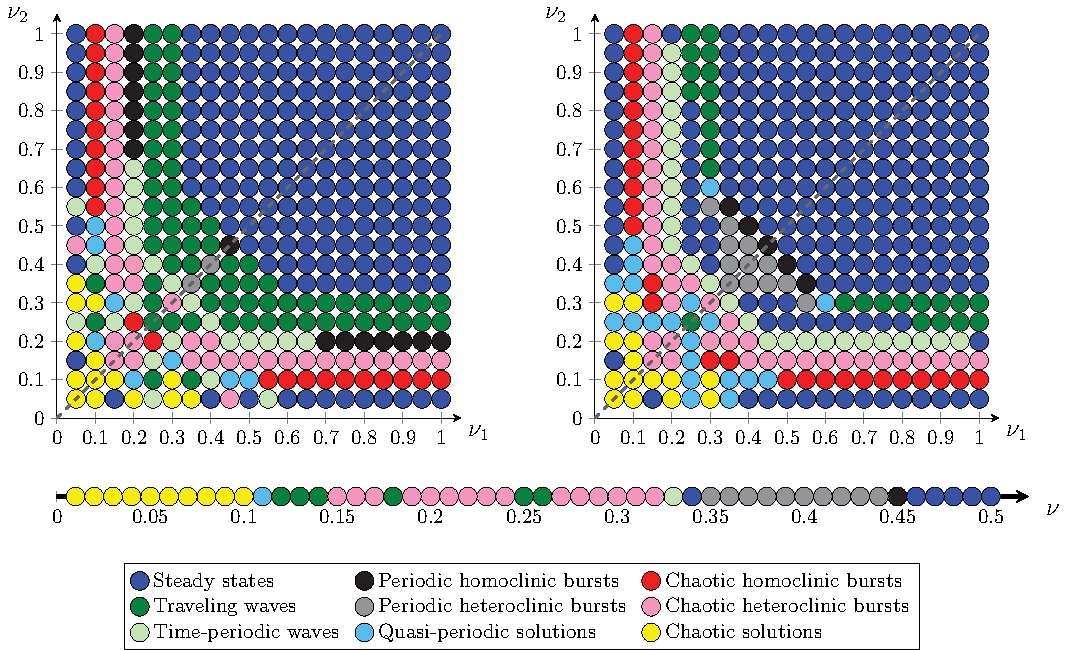
\includegraphics[width=\textwidth]{../images/nu1-nu2_presentation.pdf}
  \end{figure}
  \vspace{-0.15cm}
  \scalebox{0.4}{The top left figure is taken from \cite{Kalogirou2015}.}
\end{frame}
\begin{frame}{Results - Travelling waves}
  \begin{minipage}{0.48\textwidth}
    \centering
    $\nu_1=0.35$, $\nu_2=0.3$

    \vspace{1.5cm}
    \begin{figure}[ht]
      \centering
      \href{run:videos/animation_0.85_0.3.mp4}{
        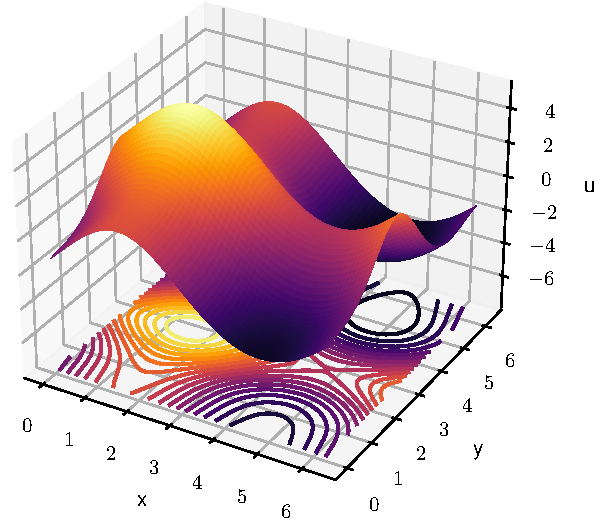
\includegraphics[width=\linewidth]{../images/slice_nu1_0.85_nu2_0.3_time_900.0.pdf}
      }
      \vspace{-0.3cm}
      \caption{\scalebox{\scalecaption}{Solution at $t=900$}}
    \end{figure}
  \end{minipage}
  \begin{minipage}{0.48\textwidth}
    \begin{itemize}
      \item Periodic in both space and time.
      \item Energy constant.
    \end{itemize}

    \vspace{1.5cm}
    \centering
    \begin{figure}[ht]
      \centering
      \href{run:videos/animation_0.4_0.4.mp4}{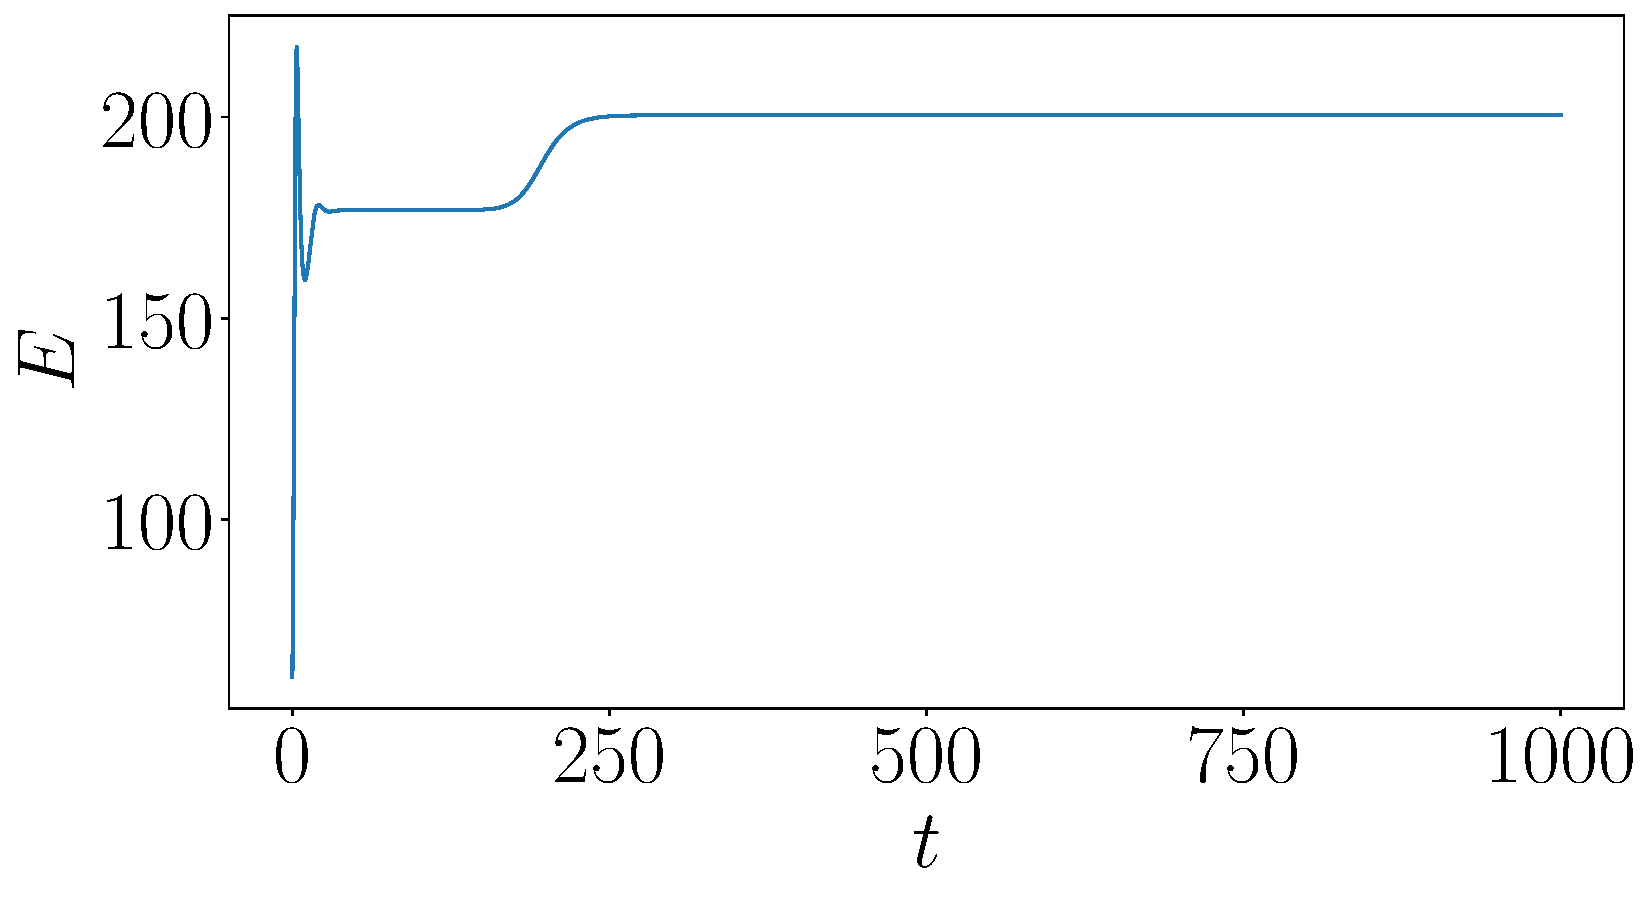
\includegraphics[width=\textwidth]{../images/tw_energy.pdf}}
      \caption{\scalebox{\scalecaption}{Energy evolution}}
    \end{figure}
  \end{minipage}
\end{frame}
\begin{frame}{Results - Time-periodic waves}
  \begin{minipage}{0.48\textwidth}
    \centering
    $\nu_1=0.35$, $\nu_2=0.3$

    \vspace{1.5cm}
    \begin{figure}[ht]
      \centering
      \href{run:videos/animation_0.35_0.3.mp4}{
        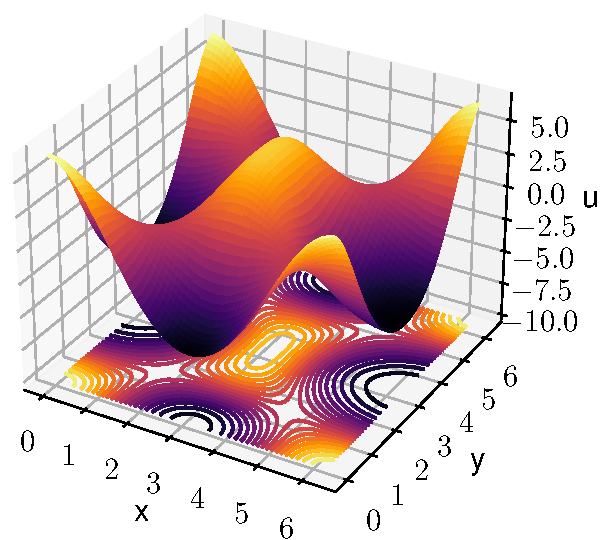
\includegraphics[width=\linewidth]{../images/slice_nu1_0.35_nu2_0.3_time_493.61.pdf}
      }
      \caption{\scalebox{\scalecaption}{Solution at $t=493.61$}}
    \end{figure}
  \end{minipage}
  \begin{minipage}{0.48\textwidth}
    \centering
    \begin{figure}[ht]
      \centering
      \href{run:videos/animation_0.4_0.4.mp4}{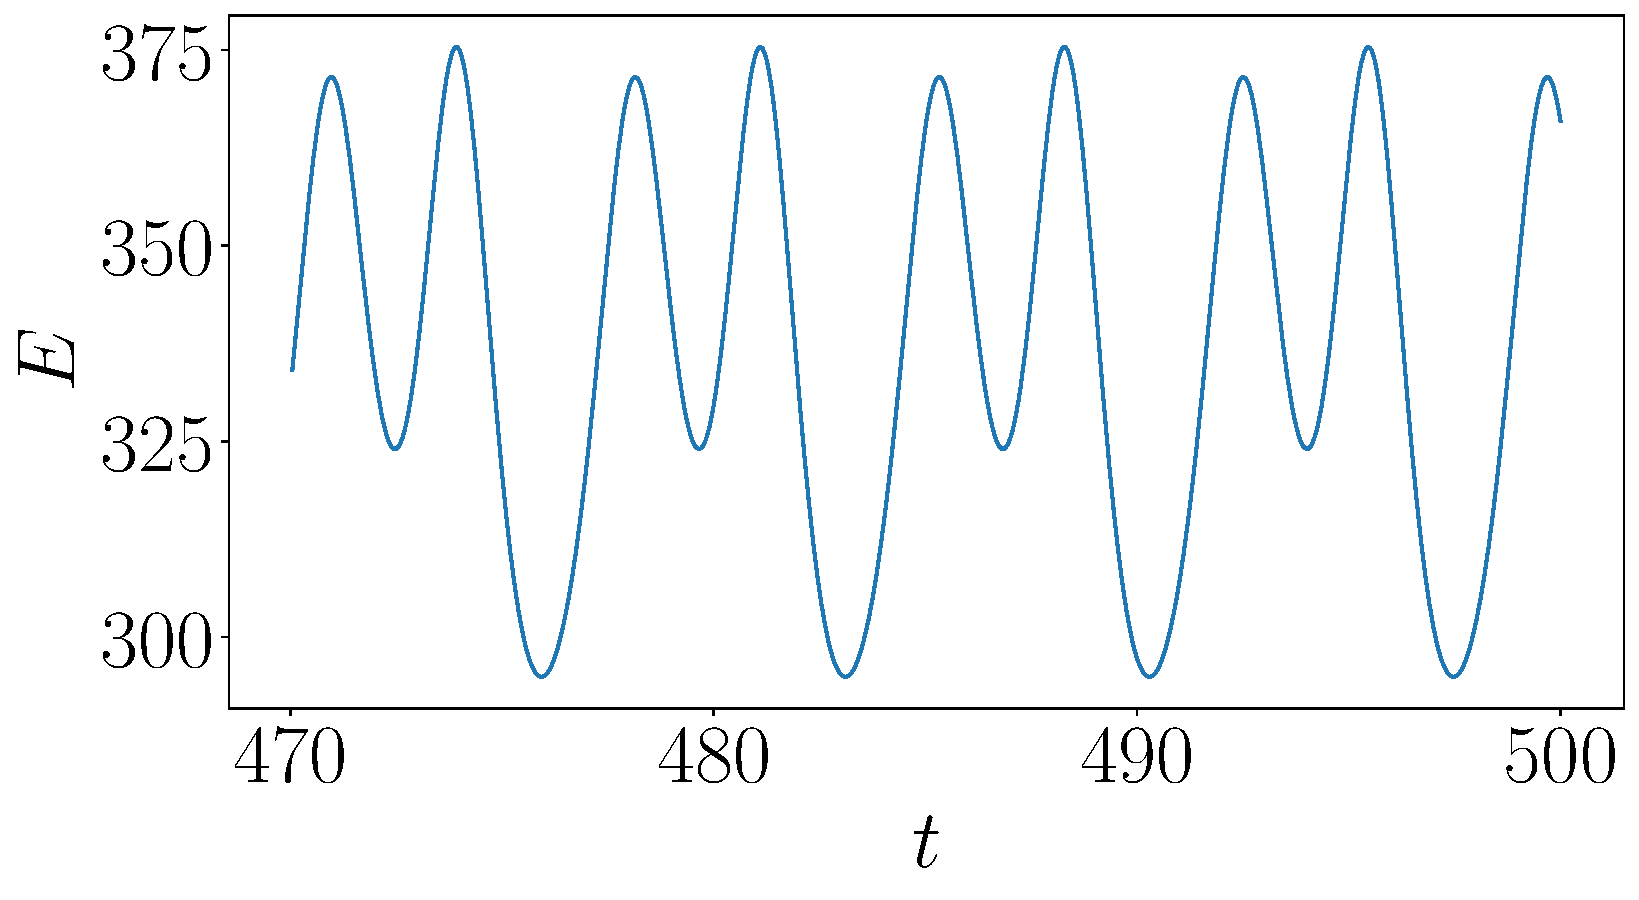
\includegraphics[width=\textwidth]{../images/tp_energy.pdf}}
      \caption{\scalebox{\scalecaption}{Energy evolution}}
    \end{figure}

    \vspace{0.2cm}
    \begin{figure}[ht]
      \centering
      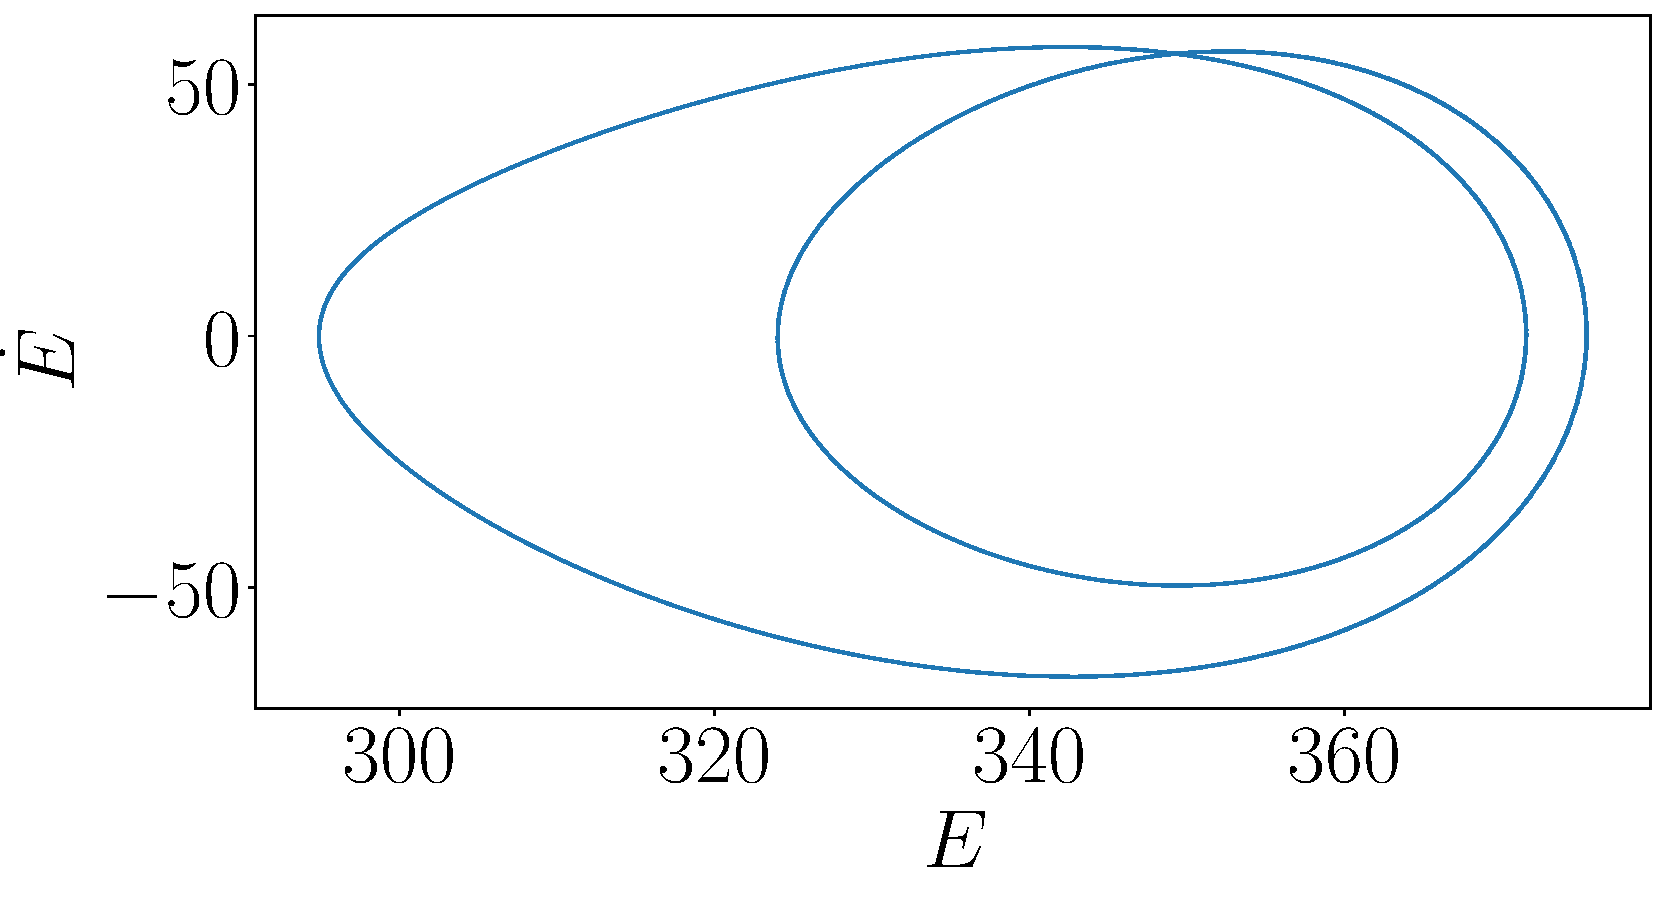
\includegraphics[width=\textwidth]{../images/tp_energy_phase.pdf}
      \caption{\scalebox{\scalecaption}{Phase space $(E,\dot{E})$}}
    \end{figure}
  \end{minipage}
\end{frame}
\begin{frame}{Results - Periodic bursts}
  \begin{minipage}{0.48\textwidth}
    \centering
    \textbf{Homoclinic burst}
    $\nu_1=\nu_2=0.45$

    \vspace{0.5cm}
    \begin{figure}[ht]
      \centering
      \href{run:videos/animation_0.45_0.45.mp4}{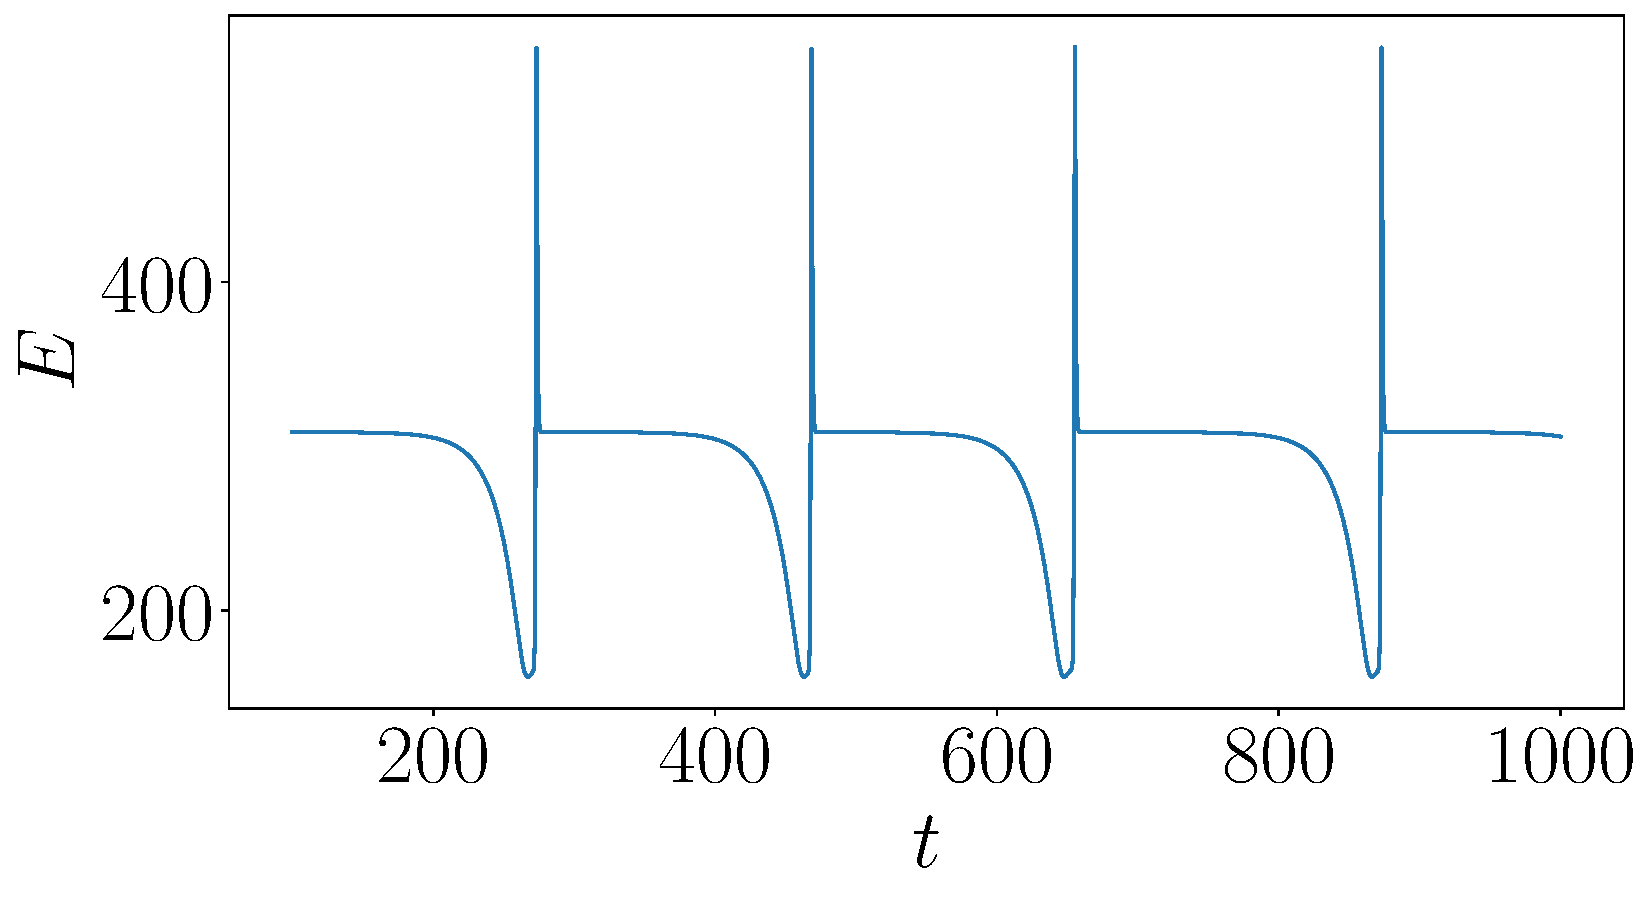
\includegraphics[width=0.9\textwidth]{../images/homo_burst.pdf}}
      \vspace{-0.3cm}
      \caption{\scalebox{\scalecaption}{Energy evolution}}
    \end{figure}
    \begin{figure}[ht]
      \centering
      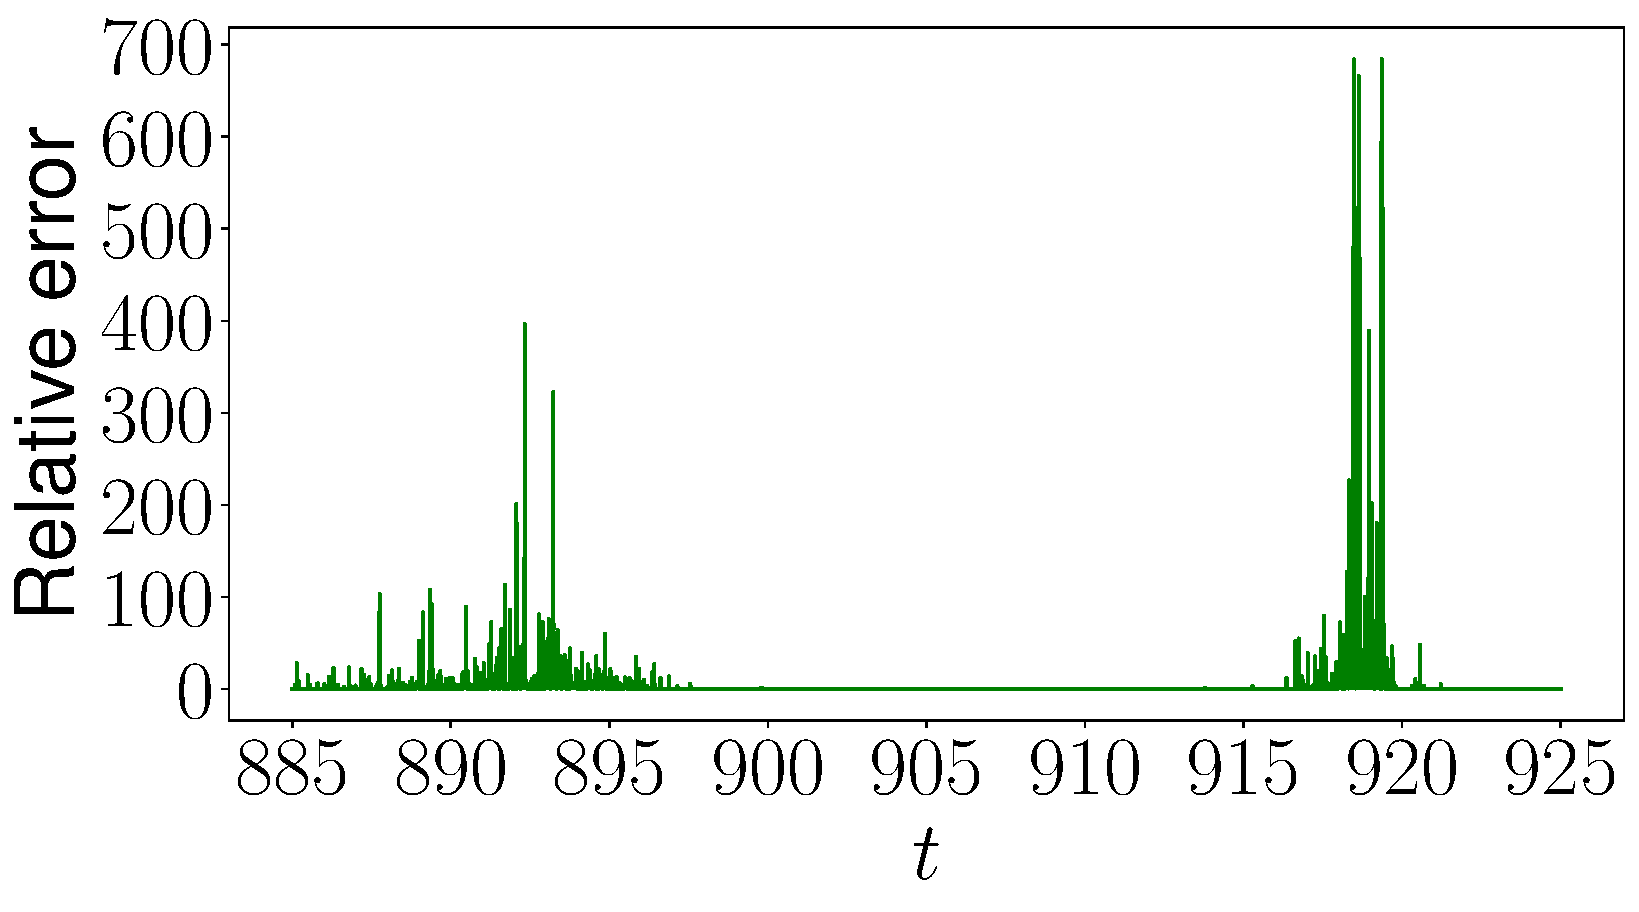
\includegraphics[width=0.9\textwidth]{../images/burst_nu1=0.40_nu2=0.40.pdf}
      \caption{\scalebox{\scalecaption}{Relative error $\displaystyle\max_{x,y\in [0,2\pi]} \frac{\abs{u(t,x,y)-u(t-h,x,y)}}{\abs{u(t,x,y)}}$}}
    \end{figure}
  \end{minipage}
  \begin{minipage}{0.48\textwidth}
    \centering
    \textbf{Heteroclinic burst}
    $\nu_1=\nu_2=0.4$
    \vspace{0.5cm}
    \begin{figure}[ht]
      \centering
      \href{run:videos/animation_0.4_0.4.mp4}{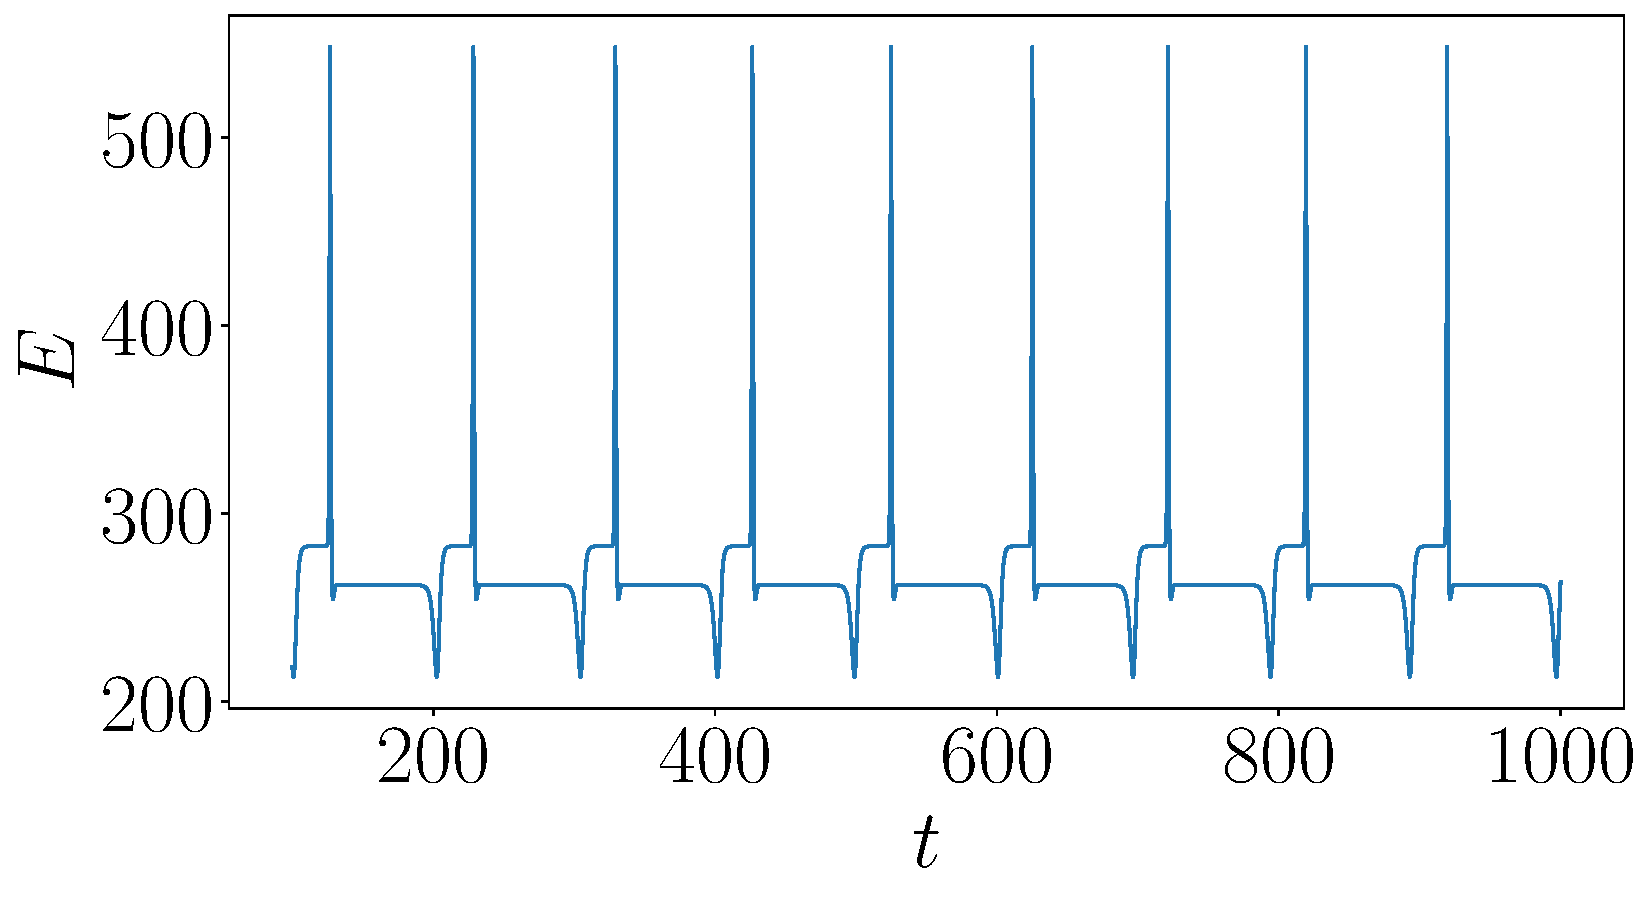
\includegraphics[width=0.9\textwidth]{../images/hetero_burst.pdf}}
      \vspace{-0.3cm}
      \caption{\scalebox{\scalecaption}{Energy evolution}}
    \end{figure}
    \begin{figure}[ht]
      \centering
      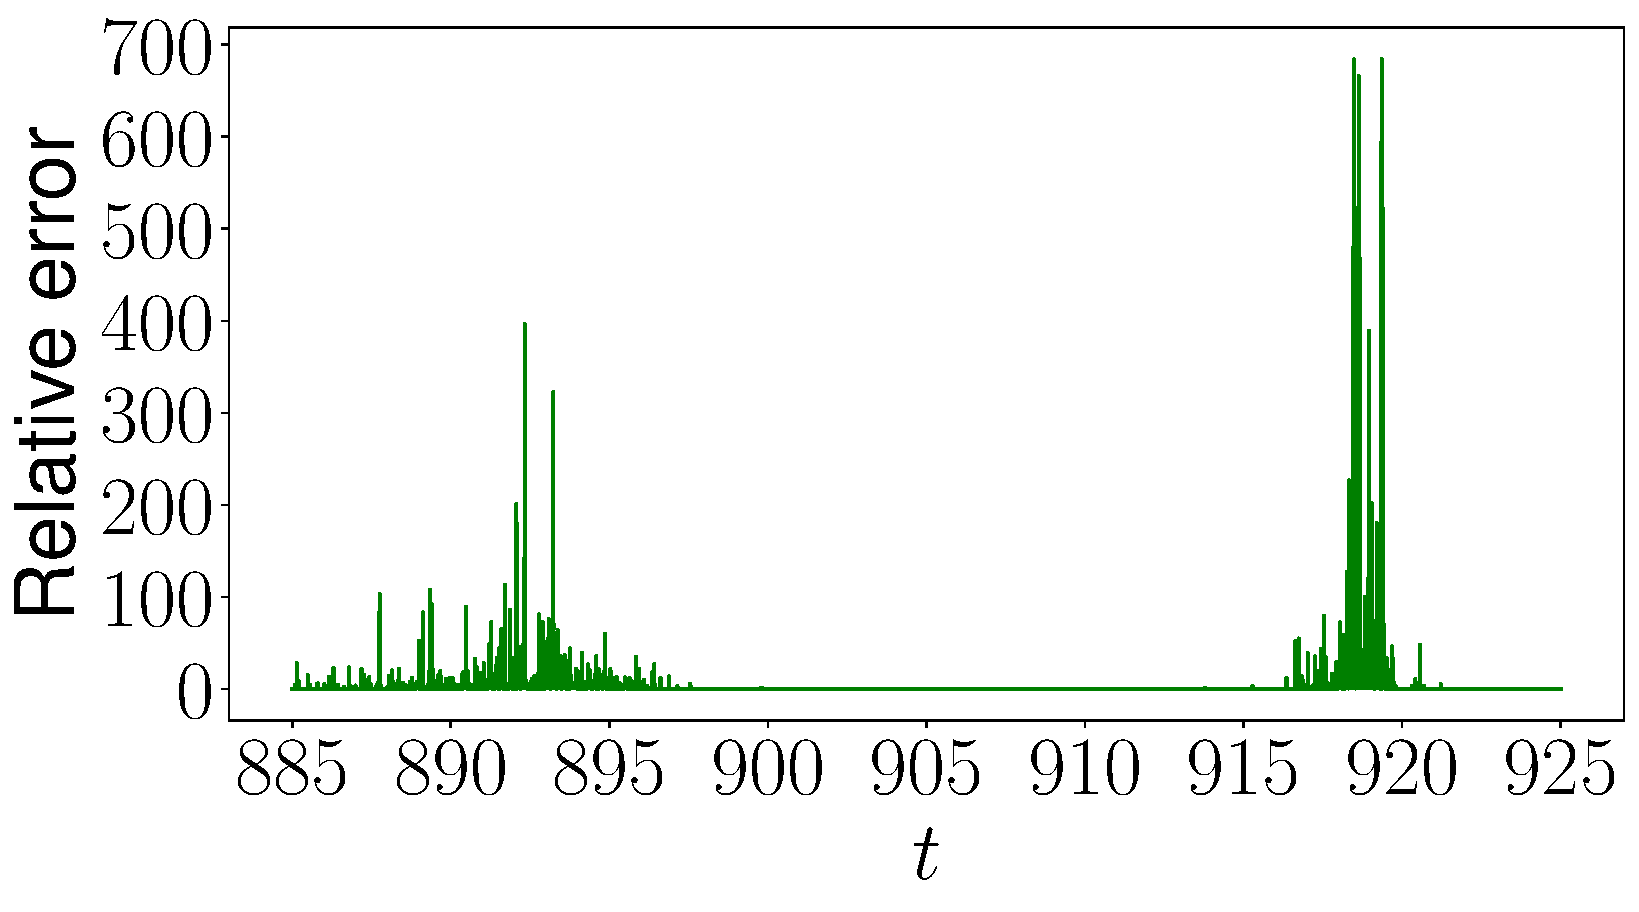
\includegraphics[width=0.9\textwidth]{../images/burst_nu1=0.40_nu2=0.40.pdf}
      \caption{\scalebox{\scalecaption}{Relative error $\displaystyle\max_{x,y\in [0,2\pi]} \frac{\abs{u(t,x,y)-u(t-h,x,y)}}{\abs{u(t,x,y)}}$}}
    \end{figure}
  \end{minipage}
\end{frame}
\begin{frame}{Results - Chaotic solutions}
  \begin{minipage}{0.48\textwidth}
    \centering
    \textbf{Quasi-periodic}

    $\nu_1=0.25$, $\nu_2=0.2$

    \vspace{0.5cm}
    \begin{figure}[ht]
      \centering
      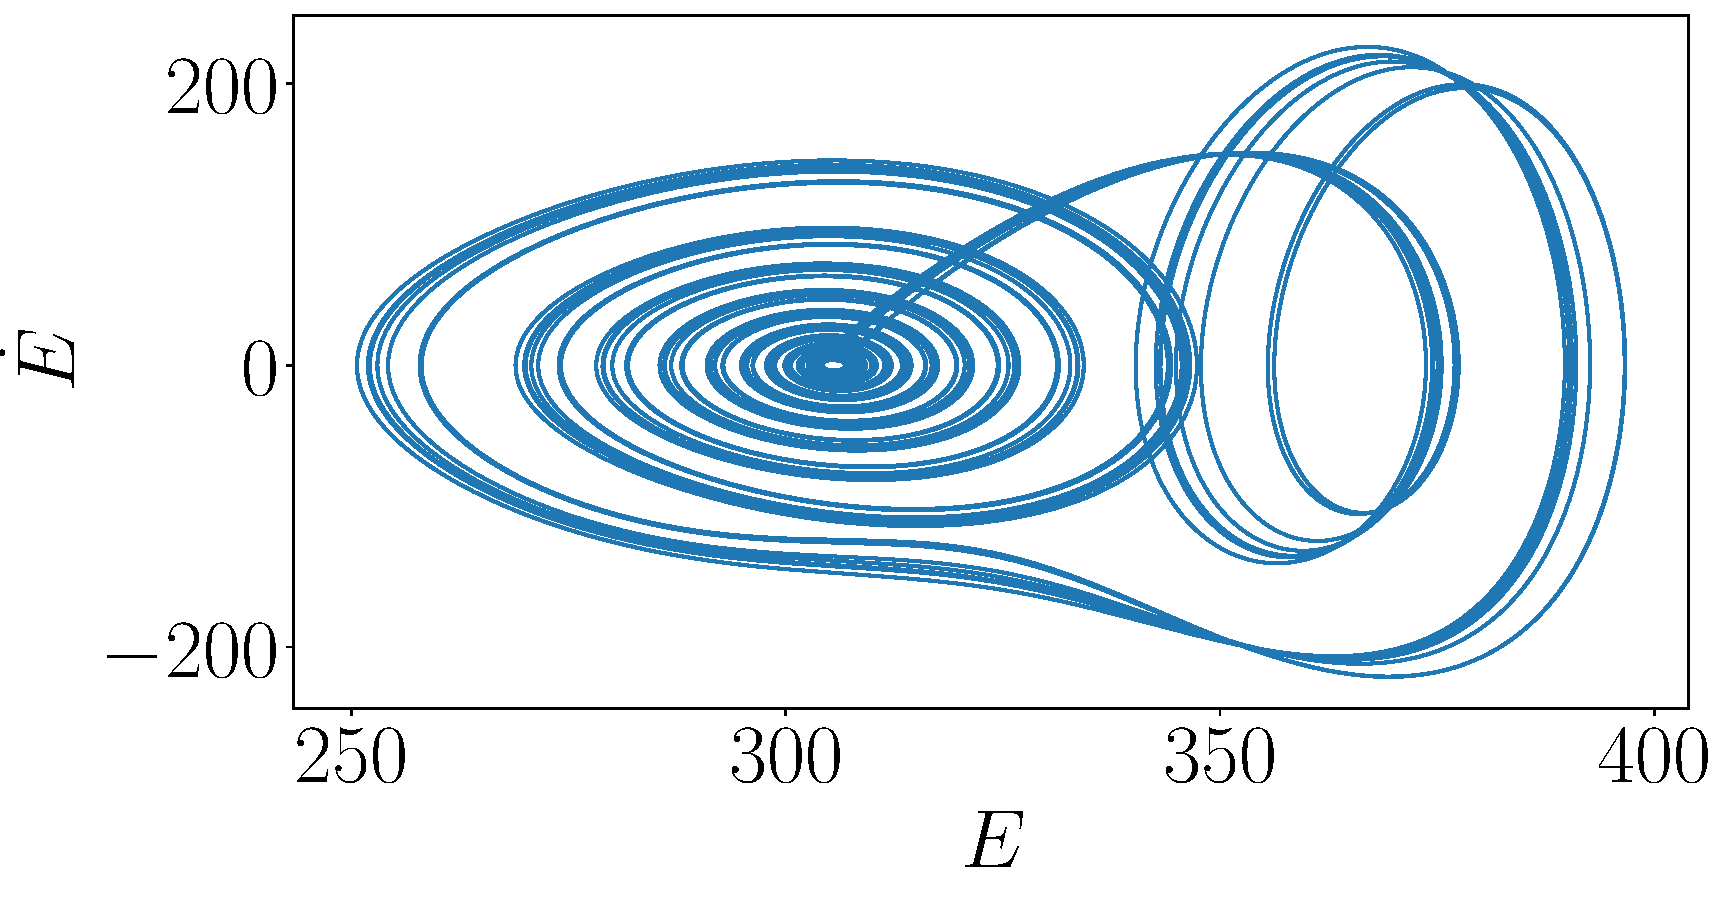
\includegraphics[width=0.9\textwidth]{../images/qp_phase.pdf}
      \vspace{-0.3cm}
      \caption{\scalebox{\scalecaption}{Phase space $(E,\dot{E})$}}
    \end{figure}

    \vspace{0.2cm}
    \begin{figure}[ht]
      \centering
      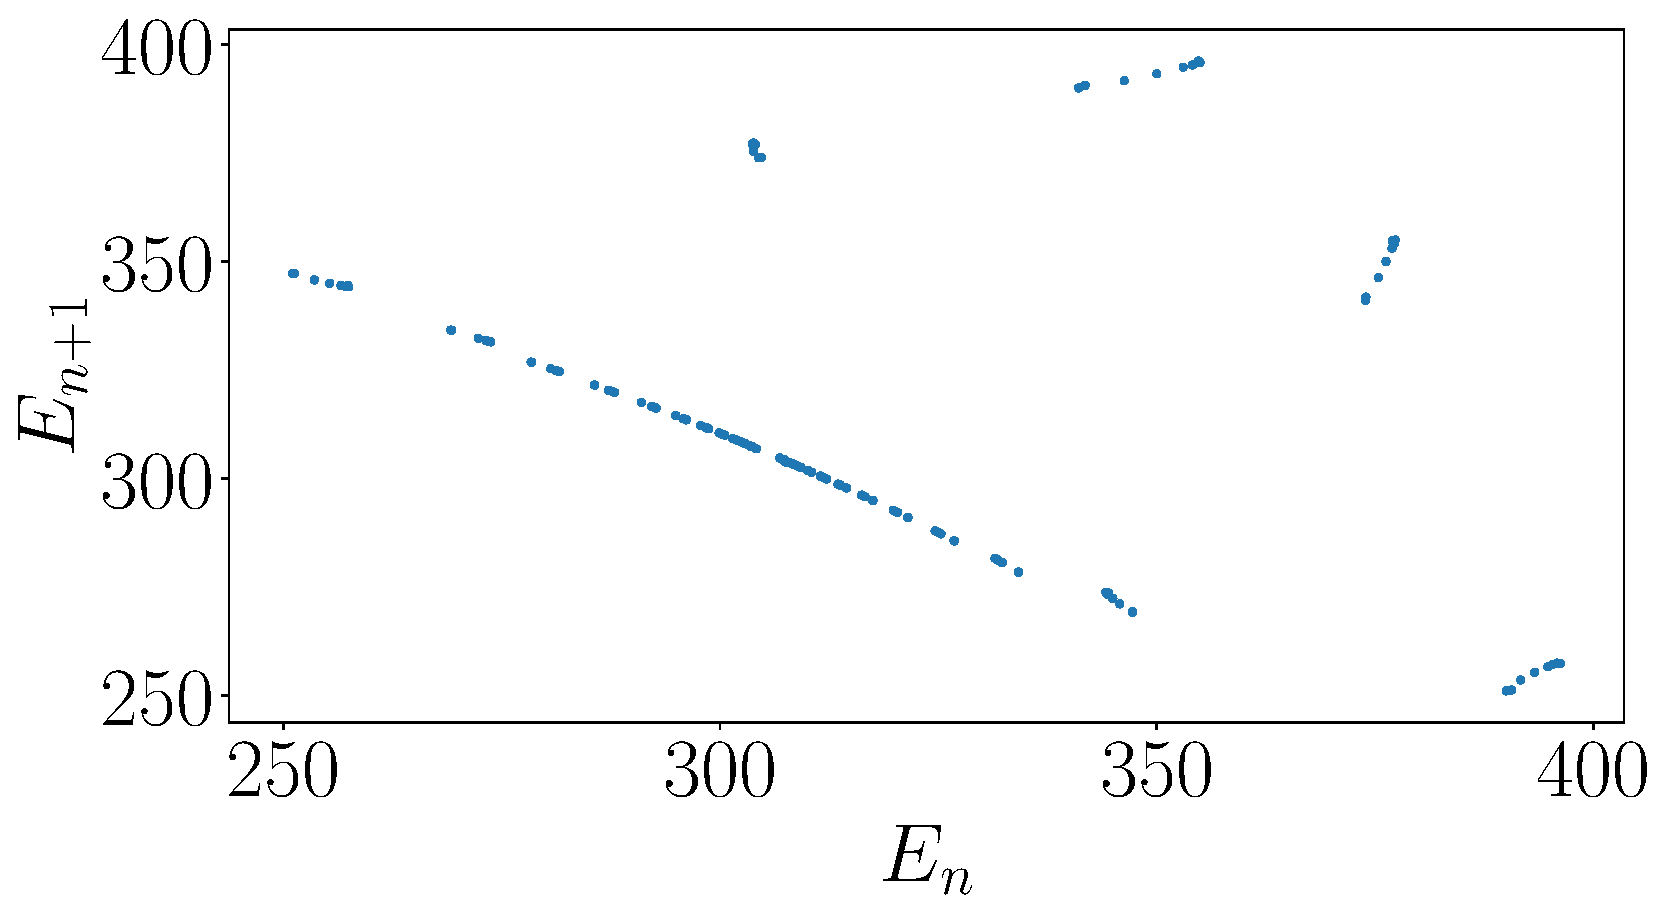
\includegraphics[width=0.9\textwidth]{../images/qp_return.pdf}
      \caption{\scalebox{\scalecaption}{Return map with section $\dot{E}=0$}}
    \end{figure}
  \end{minipage}
  \begin{minipage}{0.48\textwidth}
    \centering
    \textbf{Chaotic solution}
    $\nu_1=\nu_2=0.008$

    \vspace{0.2cm}
    \begin{figure}[ht]
      \centering
      \href{run:videos/animation_0.008_0.008.mp4}{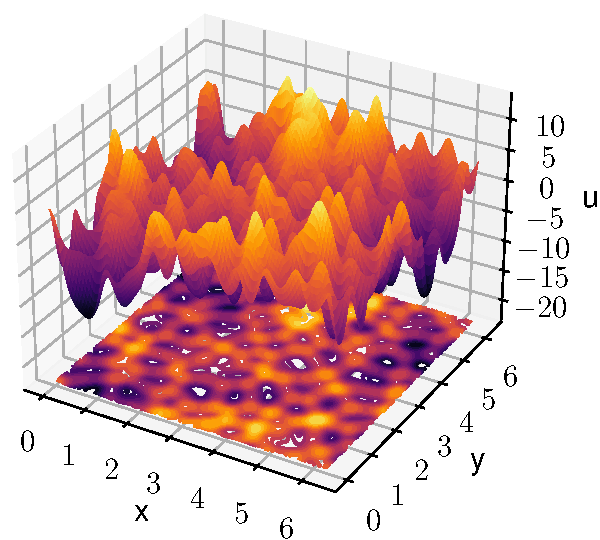
\includegraphics[width=0.62\textwidth]{../images/slice_nu1_0.008_nu2_0.008_time_5.0.pdf}}
      \vspace{-0.3cm}
      \caption{\scalebox{\scalecaption}{Solution at time $t=5$}}
    \end{figure}
    \begin{figure}[ht]
      \centering
      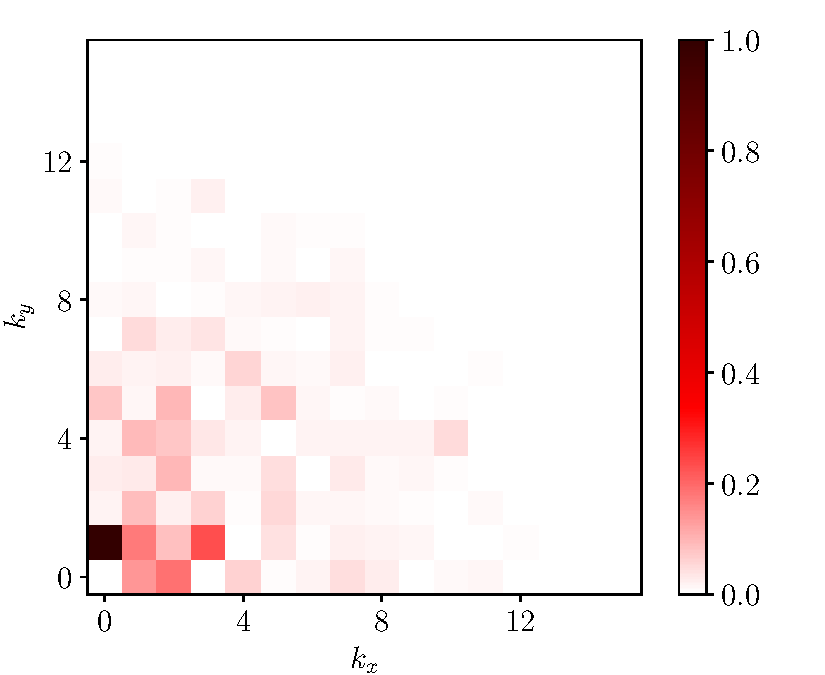
\includegraphics[width=0.62\textwidth]{../images/slice_freq_nu1_0.008_nu2_0.008_time_5.0.pdf}
      \caption{\scalebox{\scalecaption}{Fourier spectrum at time $t=5$}}
    \end{figure}
  \end{minipage}
\end{frame}
\begin{frame}{Conclusions}
  \begin{itemize}
    \item Periods of time-periodic waves are generally much smaller than periods of travelling waves and these are much smaller than periods of periodic bursts.
    \item A finer mesh grid is needed in a vicinity of bursts, specially for chaotic homoclinic and heteroclinic bursts.
    \item Quasi-periodic seem to be a transition between travelling waves or time-periodic waves and periodic bursts.
  \end{itemize}
\end{frame}
\begin{frame}[noframenumbering]{References}
  \printbibliography[heading=none]
\end{frame}
\end{document}